\documentclass[tikz,border=8pt]{standalone}
\usetikzlibrary{arrows.meta,calc,backgrounds,positioning}
\definecolor{route}{RGB}{31,78,121}
\definecolor{gate}{RGB}{196,64,44}
\definecolor{corefill}{RGB}{233,239,247}
\definecolor{outside}{RGB}{120,120,120}
\begin{document}
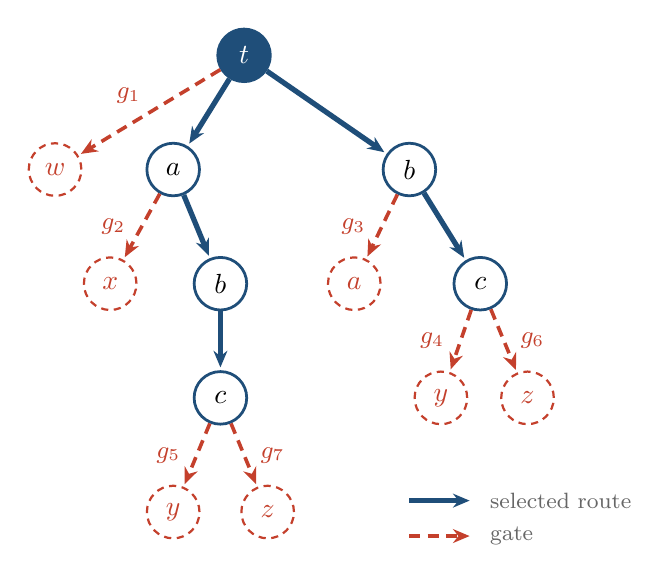
\begin{tikzpicture}[
  >={Stealth[length=6pt,width=5pt]},
  vertex/.style={circle,minimum size=19pt,inner sep=0pt,font=\normalsize},
  core/.style={vertex,draw=route,fill=white,line width=1pt},
  target/.style={vertex,draw=route,fill=route,text=white,line width=1pt},
  gnode/.style={vertex,draw=gate,fill=white,line width=0.8pt,text=gate,
                dash pattern=on 2.6pt off 2pt},
  routeedge/.style={route,line width=1.9pt,->,shorten >=1pt},
  gateedge/.style={gate,line width=1.3pt,dash pattern=on 4pt off 2.6pt,->,shorten >=1pt},
  glabel/.style={gate,font=\small},
  note/.style={font=\footnotesize,text=black!60}
]
\def\dy{1.45}
% selected states (nodes of the routing), labelled by endpoint
\node[target] (r)    at (0,0)            {$t$};
\node[core]   (a)    at (-0.9,-\dy)      {$a$};
\node[core]   (b)    at (2.1,-\dy)       {$b$};
\node[core]   (ab)   at (-0.3,-2*\dy)    {$b$};
\node[core]   (bc)   at (3.0,-2*\dy)     {$c$};
\node[core]   (abc)  at (-0.3,-3*\dy)    {$c$};
% gates: omitted extensions, labelled by the vertex they would step to
\node[gnode]  (w)    at (-2.4,-\dy)      {$w$};
\node[gnode]  (ax)   at (-1.7,-2*\dy)    {$x$};
\node[gnode]  (ba)   at (1.4,-2*\dy)     {$a$};
\node[gnode]  (bcy)  at (2.5,-3*\dy)     {$y$};
\node[gnode]  (bcz)  at (3.6,-3*\dy)     {$z$};
\node[gnode]  (abcy) at (-0.9,-4*\dy)    {$y$};
\node[gnode]  (abcz) at (0.3,-4*\dy)     {$z$};

% route edges
\draw[routeedge] (r)--(a);
\draw[routeedge] (r)--(b);
\draw[routeedge] (a)--(ab);
\draw[routeedge] (b)--(bc);
\draw[routeedge] (ab)--(abc);

% gate edges
\draw[gateedge] (r)--(w)      node[glabel,pos=0.5,above left=-1pt] {$g_1$};
\draw[gateedge] (a)--(ax)     node[glabel,pos=0.5,left=2pt] {$g_2$};
\draw[gateedge] (b)--(ba)     node[glabel,pos=0.5,left=2pt] {$g_3$};
\draw[gateedge] (bc)--(bcy)   node[glabel,pos=0.5,left=2pt] {$g_4$};
\draw[gateedge] (bc)--(bcz)   node[glabel,pos=0.5,right=2pt] {$g_6$};
\draw[gateedge] (abc)--(abcy) node[glabel,pos=0.5,left=2pt] {$g_5$};
\draw[gateedge] (abc)--(abcz) node[glabel,pos=0.5,right=2pt] {$g_7$};



% legend
\begin{scope}[shift={(2.1,-3.9*\dy)}]
\draw[routeedge] (0,0)--(0.8,0);
\node[note,anchor=west] at (0.9,0) {selected route};
\draw[gateedge] (0,-0.45)--(0.8,-0.45);
\node[note,anchor=west] at (0.9,-0.45) {gate};
\end{scope}
\end{tikzpicture}
\end{document}
